\section{Dependence of geometry estimators on hard scattering kinematics in p+Pb collisions}

Just like A+A collisions, hard-process rates in $p$+A collisions are studied as a function of centrality, defined using global event-level observables sensitive to collision geometry. In the presence of a hard scattering, however, the proton
configuration can modify the relation between those observables and the impact
parameter, contaiminatign the above correlation.
Measuring the estimators directly as a function of the reconstructed partonic kinematics inverts the usual centrality-selected approach and quantifies this bias.

This chapter presents the first measurment of event
geometry estimators on hard-scattering kinematics in $p$+Pb collisions.
Dijets are used as a proxy for the initial-state partonic scattering
configuration~\cite{HION-2023-05} and their kinematics are correlated with the Pb-going flow
forward transverse energy and zero-degree netral energy.

\subsection{Measured Observables}

The measured observables are the neutral energy deposited in the Pb-going Zero Degree
Calorimeter (ZDC), \EZDC, and the transverse energy measured in the Pb-going
Forward Calorimeter (FCal), \ETPB. The ZDC is sensitive primarily to spectator
neutrons emitted during nuclear breakup, whereas the FCal transverse energy is
an event-activity estimator sensitive to particle production by the collision
participants. Both quantities have been used to characterize the geometry of
proton--nucleus collisions.

The hard-scattering kinematics are accessed using the two highest-transverse
momentum jets in each event. The momentum fraction carried by the parton in the
proton is estimated at leading order as
\begin{equation}
    \label{eq:geometry_xp}
    x_p = \frac{p_{\mathrm{T},1}e^{y^{\mathrm{CM}}_1}
    + p_{\mathrm{T},2}e^{y^{\mathrm{CM}}_2}}
    {\sqrt{s_{\mathrm{NN}}}},
\end{equation}
where $p_{\mathrm{T},1}$ and $p_{\mathrm{T},2}$ are the transverse momenta of
the leading and subleading jets and $y^{\mathrm{CM}}_1$ and
$y^{\mathrm{CM}}_2$ are their rapidities in the nucleon--nucleon
center-of-mass frame. This estimator reconstructs the Bjorken-$x$ of the
scattered proton parton from final-state jet kinematics. Simulation studies
show that the reconstructed quantity is, on average, $6$--$8\%$ lower than the
parton-level value in the measurement phase space, with a relative resolution
that improves from about $10\%$ at low $x_p$ to $4\%$ at high $x_p$.

Normalized \EZDC\ and \ETPB\ distributions are measured in intervals of $x_p$,
along with their means, \AZDC\ and \EATPB\. The distributions expose changes in
shape, while the means provide compact measures of the $x_p$ dependence. The
correlation between \EZDC\ and \ETPB\ is also studied in each $x_p$ interval to
connect the spectator-neutron and participant-activity observables.

\subsection{Dataset and Event Selection}

\subsubsection{2016 \texorpdfstring{\pxPb}{p+Pb} Data}
The \pxPb\ data at \SNN~=~8.16~\TeV\ used for this analysis were delivered by the LHC to ATLAS in November and December of 2016. In \pxPb\ collisions at 8.16 \TeV\ the colliding beams have different energies per nucleon (6.5~\TeV\ protons colliding with $(Z/A)\times 6.5~\TeV\simeq 2.6~\TeV$ per nucleon in a lead nucleus), resulting in a collision system with \SNN~=~8.16~\TeV\ per nucleon pair. Under these conditions, the center-of-mass frame is shifted in rapidity, \RAP, by $\Delta\RAP=0.465$ in the direction of the proton beam. Data were collected in two different periods, characterized by opposite beam orientations. Due to technical issues with the ZDC instrumentation (see Section~\ref{sec:missing_zdc_mod}), only \textbf{Period B} was used for this measurement.

The runs in this period were characterized by a total integrated luminosity of 55.9~\NB. Beam 1 consisted of protons and Beam 2 of Pb ions. The protons traveled toward negative rapidities in the ``A$\rightarrow$C'' direction, corresponding to clockwise motion in the accelerator according to ATLAS conventions. This is denoted as the \pxPb\ configuration. All data sets used in this analysis, listed in Table~\ref{tab:datasets}, were processed using \textsc{ATHENA}~Release~21.

\begin{table}[ht]
    \centering
    \begin{tabular}{ | c | c |}
        \hline
        \rule{0pt}{2.25ex}
        \textbf{2016 \SNN\ = 8.16 \TeV\ Data Samples}  & \textcolor{black}{ \textbf{Luminosity [nb$^{-1}$] } } \\
        \hline
        \hline
        data16\_hip8TeV.00313063.physics\_Main.merge.AOD.r11416\_p3868 & 0.021 \\
        \hline
        data16\_hip8TeV.00313067.physics\_Main.merge.AOD.r11416\_p3868 & 0.486 \\
        \hline
        data16\_hip8TeV.00313100.physics\_Main.merge.AOD.r11416\_p3868 & 8.787 \\
        \hline
        data16\_hip8TeV.00313107.physics\_Main.merge.AOD.r11416\_p3868 & 11.053 \\
        \hline
        data16\_hip8TeV.00313136.physics\_Main.merge.AOD.r11416\_p3868 & 9.602 \\
        \hline
        data16\_hip8TeV.00313187.physics\_Main.merge.AOD.r11416\_p3868 & 3.030 \\
        \hline
        data16\_hip8TeV.00313259.physics\_Main.merge.AOD.r11416\_p3868 & 4.659 \\
        \hline
        data16\_hip8TeV.00313285.physics\_Main.merge.AOD.r11416\_p3868 & 4.272 \\
        \hline
        data16\_hip8TeV.00313295.physics\_Main.merge.AOD.r11416\_p3868 & 9.923 \\
        \hline
        data16\_hip8TeV.00313333.physics\_Main.merge.AOD.r11416\_p3868 & 3.791 \\
        \hline
        data16\_hip8TeV.00313435.physics\_Main.merge.AOD.r11416\_p3868 & 0.301 \\
        \hline
        \hline
    \end{tabular}
    \caption{\textcolor{black}{Data samples from \SNN\,= 8.16 \TeV\,\pxPb\,collisions collected during the 2016 Heavy Ion Run. The luminosity collected for each run is reported. All the data were processed using \textsc{ATHENA}~Release~21.}}
    \label{tab:datasets}
\end{table}

\subsubsection{Trigger Configuration}

\subsubsection{Monte Carlo Samples}

In order to evaluate the performance of jet reconstruction and the jet response within ATLAS, dijet Monte Carlo samples generated using \pythia~\cite{Bierlich:2022pfr} with the A14 tune and the NNPDF23LO PDFs~\cite{Ball:2012cx} were produced. Dijet events are filtered using the JZ$*$R04 filters, which select events containing an \antikt\~R~=~0.4 jet in specific truth \PT{} ranges, refered to using the prefix `JZ' and an integer ranging from 1--5 in this analysis.
The detector response was simulated using the full ATLAS detector simulation based on the Geant4 toolkit~\cite{Agostinelli:2002hh}. For \pxPb\ collisions, Pythia8 truth events are overlaid with real minimum-bias \pxPb\ data. For each event, the Pythia generation and subsequent simulations were run with conditions matching the collected data, allowing for the simulation to account for underlying event effects in the jet reconstruction. Please note that, in this MC sample, the event activity is originated mainly from the overlay contribution, and therefore has no truth associated.





Events are required to satisfy detector and data-quality requirements, contain
at least one reconstructed primary vertex, and contain two reconstructed jets.
Fully efficient central and forward single-jet triggers with different
transverse-momentum thresholds provide coverage over the analysis phase space.
Jets are reconstructed from calorimeter towers with the anti-$k_t$ algorithm,
using E-scheme recombination and radius parameter $R=0.4$. The leading and
subleading jets are required to satisfy $p_{\mathrm{T},1}>40~\mathrm{GeV}$ and
$p_{\mathrm{T},2}>30~\mathrm{GeV}$, respectively, with
$-2.8<\eta_{1,2}<4.5$. The asymmetric pseudorapidity selection prevents the
jets from biasing the Pb-going FCal estimator.

Events with either selected jet near the disabled hadronic endcap calorimeter
sector are removed. The excluded region is enlarged by 0.4 in both
pseudorapidity and azimuth, and the corresponding efficiency is included in
the detector correction. The analysis considers the 0--90\% event-activity
interval, suppressing ultra-peripheral-collision contamination. In-time pileup
is rejected by requiring that no non-primary vertex has more than six associated
tracks. A ZDC pre-sample requirement rejects events with elevated baselines
from preceding interactions, thereby removing residual out-of-time pileup that
can distort the FCal energy measurement.

Detector effects are evaluated with \textsc{Pythia} dijet events overlaid with
minimum-bias $p$+Pb data during detector simulation. The simulated FCal
distribution is reweighted at the event level to match that of the dijet data.

\subsubsection{Missing ZDC Module on Side C}
\label{sec:missing_zdc_mod}
During the 2016 \pxPb\ run, the ZDC side C module 0 (EM) was removed and replaced with the Arm2 calorimeter of the LHCf experiment~\cite{Adriani:2135330}. Figure~\ref{fig:lhcf_v_zdc_acceptance} displays the transverse acceptance of both the ATLAS ZDC and LHCf.  The ATLAS ZDC EM Module is the first of 4 sequential calorimeter modules (counting from the perspective of looking at the ZDCs from the ATLAS interaction point); therefore, the LHCf calorimeter would see forward neutral products before they reach the side C ZDC.  The LHCf detector was put in place to measure the forward neutral products of the proton going side in the \pxPb\ orientation; however, in the \Pbxp\ orientation the LHCf detector was retracted into the ``garage'' position to avoid radiation damage~\cite{Adriani:2135330}.  The ``garage'' position indicates an upwards vertical shift of 112 mm from the nominal position shown in Figure~\ref{fig:lhcf_v_zdc_acceptance}.  This shift places the full LHCf Arm2 calorimeter outside of the full acceptance of the ATLAS ZDC.  Still, the side C ZDC suffers from only having roughly 75~\% of the material budget of side A. This effectively reduces the interaction length of the side C ZDC from 4.6 to 3.4, which in turn reduces the neutrons expected to shower in the ZDC from 99\% to 96.6\%. For this reason, in this analysis only Period B (\pxPb), is used to obtain the final results.

\begin{figure}[p]
    \centering
    \begin{subfigure}[c]{0.45\linewidth}
        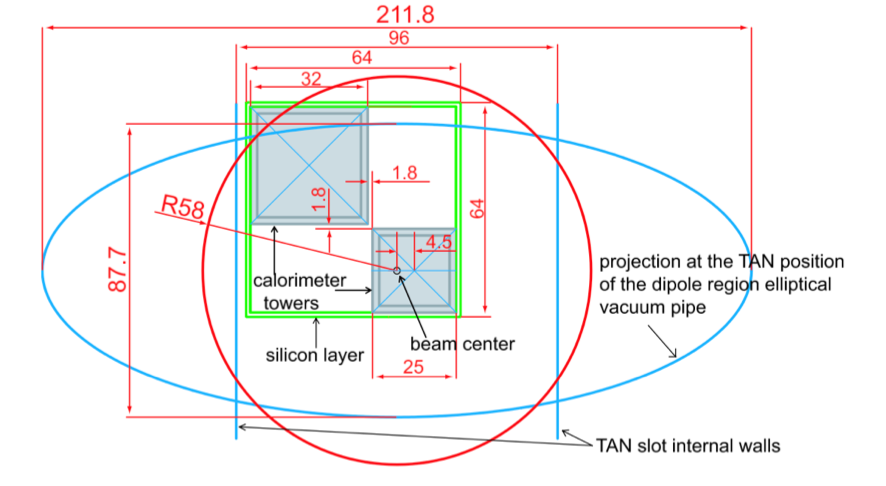
\includegraphics[
            width=1\linewidth,
            alt={Transverse acceptance of the LHCf Arm2 calorimeter viewed from the ATLAS interaction point.}
        ]{chapters/geometry_estimators_pPb/figures/dataset_and_event_selection/lhcfAcceptence.png}
    \end{subfigure}
    \begin{subfigure}[c]{0.45\linewidth}
        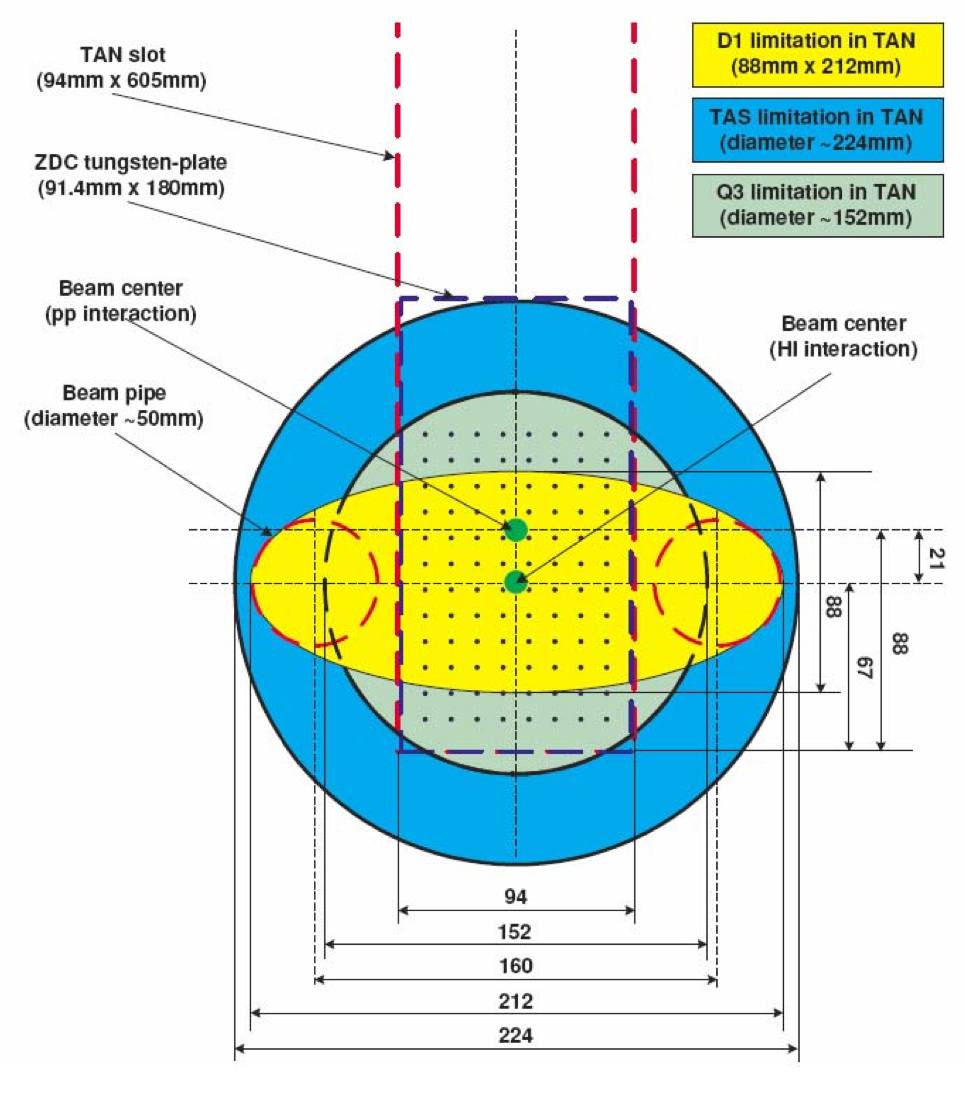
\includegraphics[
            width=1\linewidth,
            alt={Transverse acceptance of the ATLAS ZDC viewed from the ATLAS interaction point.}
        ]{chapters/geometry_estimators_pPb/figures/dataset_and_event_selection/zdcAcceptence.png}
    \end{subfigure}
    \caption{Detector Geometry for LHCf Arm2~\cite{Cekmecelioglu:2867369} (left) and the ATLAS ZDC~\cite{Jenni:1009649} (right). View is from the perspective of the ATLAS interaction point. In both figures the distances are given in mm.  The blue oval in the left image corresponds to the boundary of the yellow oval in the right image.  The active area of LHCf is represented by the filled blue squares.  The active area of the ZDC is given by the area bounded by the purple dashed line.}
    \label{fig:lhcf_v_zdc_acceptance}
\end{figure}

In the \pxPb\ orientation, the LHCf was in running position in runs 313063 and 313435, while for all other runs it was in ``garage'' position. Due to the asymmetric design of the LHCf module in the transverse plane, the effect on the acceptance of the ZDC in the proton-going direction during these runs is nontrivial. Any measurement in this thesis using the proton-going ZDC excludes these runs.

\subsection{Analysis Procedure}
\label{ssec:unf_strat}

The Pb-going FCal transverse energy is constructed by summing the transverse
projection of the electromagnetic-scale tower energies in the hemisphere facing
the Pb beam. This definition is consistent with previous ATLAS $p$+Pb
centrality measurements. In typical events containing a hard scattering, the
energy observed in the Pb-going ZDC is dominated by spectator neutrons
evaporating from the struck nucleus.

The ZDC energy scale is determined run by run from the response to a single
spectator neutron. The low-energy spectrum contains distinguishable neutron
peaks, and a simultaneous fit to the first three peaks and a background term
validates the calibration. The fitted single-neutron peak is constrained to the
nominal per-nucleon beam energy. The detector response below $1~\mathrm{TeV}$
is limited by detector noise and low-energy backgrounds; this region is treated
as a dedicated zero-energy bin. A residual in-time pileup contribution to the
\EZDC distribution is removed with a data-driven template method.

Finite jet-resolution effects cause migration in $x_p$. These effects are
corrected with a two-dimensional iterative Bayesian unfolding procedure using
RooUnfold. The response matrix contains $x_p$ and, in turn, either \EZDC or
\ETPB. Since the available simulation does not model nuclear breakup in the ZDC
or the full FCal response for the overlaid minimum-bias event, the calorimeter
observable is propagated through the unfolding with diagonal migration
matrices. This retains the measured correlation of calorimeter energy with
$x_p$ while correcting the jet-related kinematic migration.

The response matrix is reweighted as a function of reconstructed $x_p$ to
match the data spectrum. For the ZDC measurement, pileup-subtracted data
distributions are sampled to assign a ZDC energy to each simulated dijet event.
The procedure is repeated with independent random seeds, and closure tests
verify that the unfolding reproduces the particle-level simulation. Two
iterations are used, balancing the convergence of the unfolded result against
the growth of statistical uncertainty. Statistical uncertainties are evaluated
by bootstrap resampling of both the data and response matrix.

\subsection{Systematic Uncertainties}

Systematic uncertainties arise from the jet energy scale (JES), jet energy
resolution (JER), unfolding prior, disabled HEC sector, and the ZDC energy
calibration. Except for the HEC and ZDC-scale variations, the full analysis is
repeated with a response matrix modified according to each systematic
variation. The difference relative to the nominal result defines the
corresponding uncertainty.

The JES and JER variations quantify the mean and width of the
$p_{\mathrm{T}}^{\mathrm{reco}}/p_{\mathrm{T}}^{\mathrm{gen}}$ response for
matched jets. The HEC uncertainty is evaluated by enlarging the jet-exclusion
region by 0.1 in both pseudorapidity and azimuth. To test the sensitivity to
the unfolding prior, the response matrices are constructed without the nominal
event-level reweighting and the full unfolding is repeated.

The ZDC-specific uncertainty includes the stability of the single-neutron peak,
the residual energy-scale variation, and the non-linear energy correction. The
FCal stability across the data-taking period is negligible relative to the
other sources. The independent variations are added in quadrature. For ratios
between $x_p$ intervals, JES, JER, HEC, and ZDC uncertainties are treated as
fully correlated, while the unfolding-prior contribution is treated as
uncorrelated.

For the normalized distributions, the \EZDC uncertainty is typically dominated
by the ZDC energy-stability term and is below $7\%$ over most of the measured
range. The \ETPB distribution uncertainty is primarily driven by JES, JER, and
the unfolding prior and is generally below $10\%$. The systematic uncertainties
on \AZDC and \EATPB are below $2\%$ in all but the lowest $x_p$ interval.

\subsection{Results}

The normalized \ETPB and \EZDC distributions change systematically with $x_p$.
Relative to a low-$x_p$ selection, high-$x_p$ dijet events exhibit an \ETPB
distribution shifted toward lower energies. This is a direct confirmation of
the event-activity bias previously observed in centrality-dependent jet
measurements. The \EZDC distribution shows a qualitatively similar trend: at
high $x_p$, a larger fraction of events contains fewer forward neutrons. The
effect in the ZDC is, however, substantially weaker than that in the FCal.

The mean values \AZDC and \EATPB both decrease with increasing $x_p$, most
visibly for $x_p\gtrsim 0.02$, where earlier ATLAS measurements found evidence
for small proton-size configurations. Across this range, \AZDC decreases by up
to about $5\%$, corresponding on average to two fewer beam-energy neutrons,
whereas \EATPB decreases by up to $40\%$. When the two means are normalized to
their maximum values, the FCal estimator is found to be approximately six times
more sensitive to hard-process kinematics than the ZDC estimator.

The relation between \ETPB and \EZDC is also $x_p$ dependent. For ZDC energies
below approximately $150~\mathrm{TeV}$, the average FCal transverse energy is
consistent with a linear dependence on the ZDC energy in low-, middle-, and
high-$x_p$ selections. The slope decreases progressively from low to high
$x_p$, and the Pearson correlation coefficient changes by approximately $3\%$
across the measured range. At higher ZDC energies, deviations from the linear
trend are consistent with larger fluctuations in nuclear breakup for events
with the greatest event activity.

These results show that both common geometry estimators retain sensitivity to
the proton configuration associated with a hard scattering. The ZDC observable
is more robust than Pb-going FCal transverse energy, but is not independent of
the hard-scattering kinematics. This observation provides experimental input
for simultaneous descriptions of event activity, nuclear breakup, and color
fluctuations in $p$+Pb collisions.

